\documentclass[11pt,a4paper]{article}
\usepackage[T1]{fontenc}
\usepackage[utf8]{inputenc}
\usepackage{lmodern}
\usepackage[margin=2.5cm]{geometry}
\usepackage{amsmath,amssymb}
\usepackage{booktabs}
\usepackage{graphicx}
\usepackage{caption}
\usepackage[round,authoryear]{natbib}
\usepackage[hidelinks]{hyperref}
\usepackage{url}
\usepackage{microtype}
\setlength{\parskip}{3pt}
\captionsetup{font=small,labelfont=bf}
% generated by build_exhibits.py - do not edit by hand
\newcommand{\ARCHK}{0.096}
\newcommand{\ARCHR}{0.275}
\newcommand{\BICone}{\ensuremath{-}138.52}
\newcommand{\BICtwo}{\ensuremath{-}346.62}
\newcommand{\BPK}{0.853}
\newcommand{\BPR}{0.090}
\newcommand{\BaseAll}{0.353}
\newcommand{\BaseAllPct}{35}
\newcommand{\BiasaK}{2.18}
\newcommand{\BiasaR}{0.33}
\newcommand{\BiasaRatio}{1.23}
\newcommand{\BiassK}{\ensuremath{-}0.01}
\newcommand{\BiassR}{0.00}
\newcommand{\BiassRatio}{\ensuremath{-}0.01}
\newcommand{\CIaKhi}{11.68}
\newcommand{\CIaKlo}{\ensuremath{-}3.82}
\newcommand{\CIaRatiohi}{5.68}
\newcommand{\CIaRatiolo}{\ensuremath{-}1.05}
\newcommand{\CIaRhi}{5.47}
\newcommand{\CIaRlo}{0.50}
\newcommand{\CIsKhi}{0.749}
\newcommand{\CIsKlo}{0.516}
\newcommand{\CIsRatiohi}{3.40}
\newcommand{\CIsRatiolo}{2.22}
\newcommand{\CIsRhi}{0.250}
\newcommand{\CIsRlo}{0.205}
\newcommand{\CrisisEpLengths}{63, 44, 9, 8, 7, 6, 2}
\newcommand{\CrisisShareJune}{15}
\newcommand{\DBICone}{208.10}
\newcommand{\DBICtwo}{146.34}
\newcommand{\Decisive}{81.2}
\newcommand{\ETprim}{4.28}
\newcommand{\EndDate}{26 June 2026}
\newcommand{\IndepSD}{1.9}
\newcommand{\InflDacc}{0.0015}
\newcommand{\InflDlim}{0.023}
\newcommand{\Iter}{27}
\newcommand{\JBK}{<0.001}
\newcommand{\JBR}{0.42}
\newcommand{\KOne}{9}
\newcommand{\KTwo}{21}
\newcommand{\LBfiveK}{0.104}
\newcommand{\LBfiveR}{0.459}
\newcommand{\LLone}{95.96}
\newcommand{\LLtwo}{235.60}
\newcommand{\LUK}{\ensuremath{-}2.1}
\newcommand{\LUR}{\ensuremath{-}2.7}
\newcommand{\LowPa}{0.0186}
\newcommand{\LowPb}{0.0292}
\newcommand{\MeanaK}{6.26}
\newcommand{\MeanaR}{3.31}
\newcommand{\MeanaRatio}{2.60}
\newcommand{\MeanbK}{0.9756}
\newcommand{\MeansK}{0.59}
\newcommand{\MeansR}{0.22}
\newcommand{\MeansRatio}{2.65}
\newcommand{\MedAbsTen}{2.2}
\newcommand{\MinP}{0.00265}
\newcommand{\NCalmDays}{238}
\newcommand{\NCrisisDays}{139}
\newcommand{\NCrisisDaysCross}{133}
\newcommand{\NCrisisEp}{7}
\newcommand{\NDays}{377}
\newcommand{\NDaysJune}{20}
\newcommand{\NDisagree}{8}
\newcommand{\NEventDays}{25}
\newcommand{\NEvents}{26}
\newcommand{\NEventsEarly}{10}
\newcommand{\NEventsJune}{9}
\newcommand{\NEventsJuneTD}{10}
\newcommand{\NEventsLate}{16}
\newcommand{\NEventsSmallMove}{10}
\newcommand{\NEventsTD}{21}
\newcommand{\NHighEarly}{28}
\newcommand{\NHitsEarly}{4}
\newcommand{\NHitsLate}{5}
\newcommand{\NLateCrisis}{8}
\newcommand{\NLevelDays}{378}
\newcommand{\NLowP}{2}
\newcommand{\NMat}{11}
\newcommand{\NPairsAll}{376}
\newcommand{\NPairsKept}{363}
\newcommand{\NRetroHits}{3}
\newcommand{\NSeams}{13}
\newcommand{\NSeg}{14}
\newcommand{\NStarts}{24}
\newcommand{\NStartsConv}{24}
\newcommand{\NStartsIdxZero}{11}
\newcommand{\NStartsSame}{24}
\newcommand{\NSwitch}{13}
\newcommand{\NSwitchCross}{17}
\newcommand{\NSwitchEarly}{6}
\newcommand{\NSwitchJune}{3}
\newcommand{\NTagJune}{18}
\newcommand{\NTags}{58}
\newcommand{\NTagsTD}{47}
\newcommand{\NWinAprMay}{37}
\newcommand{\NWinAprMayHit}{37}
\newcommand{\NWinJune}{20}
\newcommand{\NWinJuneHit}{3}
\newcommand{\NWindowDays}{57}
\newcommand{\NbOneK}{87}
\newcommand{\NbOneR}{3}
\newcommand{\NullGE}{41}
\newcommand{\NullMax}{12}
\newcommand{\NullMin}{0}
\newcommand{\NullSD}{2.9}
\newcommand{\PCAone}{70.8}
\newcommand{\PCAsum}{99.2}
\newcommand{\PCAthree}{1.2}
\newcommand{\PCAtwo}{27.1}
\newcommand{\PCacfOne}{0.98}
\newcommand{\PCacfTwo}{0.99}
\newcommand{\PStayCalm}{0.956}
\newcommand{\PStayCrisis}{0.915}
\newcommand{\PaltSrc}{0.1114}
\newcommand{\PcritPrim}{0.0318}
\newcommand{\PhiaK}{88.02}
\newcommand{\PhiaR}{94.00}
\newcommand{\PhiaRatio}{92.64}
\newcommand{\PhisK}{99.68}
\newcommand{\PhisR}{98.77}
\newcommand{\PhisRatio}{99.16}
\newcommand{\PloaK}{0.28}
\newcommand{\PloaR}{0.90}
\newcommand{\PloaRatio}{0.65}
\newcommand{\PlosK}{8.01}
\newcommand{\PlosR}{4.44}
\newcommand{\PlosRatio}{5.35}
\newcommand{\Pprim}{0.1088}
\newcommand{\PtaK}{4.07}
\newcommand{\PtaR}{2.98}
\newcommand{\PtaRatio}{1.37}
\newcommand{\PtsK}{0.598}
\newcommand{\PtsR}{0.225}
\newcommand{\PtsRatio}{2.66}
\newcommand{\PtsRatioRound}{2.7}
\newcommand{\RMax}{2.71}
\newcommand{\RMin}{1.82}
\newcommand{\RatioCritPrim}{2.6}
\newcommand{\RatioMax}{2.48}
\newcommand{\RatioMin}{1.79}
\newcommand{\RsqShort}{0.986}
\newcommand{\SeamShare}{3.46}
\newcommand{\StartChg}{3 January 2025}
\newcommand{\StartLevel}{2 January 2025}
\newcommand{\TCK}{7.6}
\newcommand{\TCR}{4.4}
\newcommand{\TagEnd}{29 June 2026}
\newcommand{\TagHit}{0.660}
\newcommand{\TagHitEight}{0.574}
\newcommand{\TagStart}{8 April 2026}
\newcommand{\TcritPrim}{11}
\newcommand{\Tobs}{9}
\newcommand{\TrCalm}{0.133}
\newcommand{\TrCrisis}{0.568}
\newcommand{\WinHit}{0.702}
\newcommand{\aK}{4.07}
\newcommand{\aR}{2.98}
\newcommand{\bK}{0.98397}
\newcommand{\bR}{0.98824}
\newcommand{\nK}{132}
\newcommand{\nR}{231}
\newcommand{\sK}{0.598}
\newcommand{\sR}{0.225}

\makeatletter\newcommand{\tabinput}[1]{\@@input #1 }\makeatother

\title{Regime-Switching Short-Rate Dynamics:\\ A Hidden Markov Approach to Hull--White Estimation\\ on Euro-Area Government Bond Yields}
\author{Klaus Leopold von Moltke\thanks{DHBW Mannheim (BWL--Versicherung). Working paper, 1 October 2026. Code and data availability and the use of AI assistance are stated at the end of the paper. \copyright{} 2026 Klaus Leopold von Moltke. This paper is licensed under CC~BY~4.0 (\url{https://creativecommons.org/licenses/by/4.0/}); the accompanying code is licensed under the MIT License.}}
\date{Working paper -- 1 October 2026}

\begin{document}
\maketitle

\begin{abstract}
\noindent
This paper asks two falsifiable questions on ECB estimates of \NLevelDays{} daily euro-area AAA government yield curves (\StartLevel{} to \EndDate{}). (a) Do regimes that a two-state Gaussian hidden Markov model infers blindly from daily changes in level, slope and curvature coincide with \NEvents{} monetary-policy, geopolitical, macroeconomic and fiscal events more closely than chance? (b) Conditional on the inferred regimes, do the short-rate parameters of a one-factor Hull--White (Ornstein--Uhlenbeck) model, estimated under the physical measure from the 3-month rate, differ across regimes beyond estimation uncertainty, and is the regime-conditional specification preferred? The test design for (a), including its significance level and a stopping rule, was fixed in dated project documents before the test was run, as were the main elements of the estimation design for (b). For (a), an exact circular-shift (rotation) test finds $T_{\mathrm{obs}}=\Tobs$ events within two trading days of a regime transition against $\ETprim$ expected under the null ($p=\Pprim$); the pre-registered primary test is not significant, and the result is reported as a negative result with a diagnosis. For (b), short-rate volatility in the high-volatility (`crisis') regime is \PtsRatio{} times that in the low-volatility (`calm') regime (95\% BCa interval [\CIsRatiolo, \CIsRatiohi]), a difference that the variance-based regime definition partly implies; conditional on the regime path, BIC prefers the regime-specific model. The mean-reversion speed cannot be estimated precisely at this sample length, so the pre-registered joint claim that both parameters differ is not made. The results suggest that yield-only Gaussian regimes separate volatility states but cannot, on about 18 months of data, be tied to economic events beyond the chance alignment of two clustered series.
\end{abstract}

\section{Introduction}\label{sec:intro}

Single-regime short-rate models such as Hull--White let their parameters vary, if at all, as deterministic functions of time that are fixed when the model is fitted \citep[eq.~3]{hullwhite1990}; the dynamics cannot switch with an unobserved economic state. Euro-area interest rates in 2025--2026, however, moved through a sequence of monetary-policy turns and geopolitical shocks that a single parameter set can absorb only crudely. Regime-switching models address this by letting an unobserved state, which follows a first-order Markov chain, govern the dynamics \citep[p.~357 and eq.~2.2]{hamilton1989}. For interest rates, such models are well suited to capture non-linearities, and single-regime specifications are clearly rejected against them \citep[abstract and p.~2]{angbekaert1998}. Regime shifts have also been built into arbitrage-free term-structure models, with regime-dependent market prices of risk \citep{bansalzhou2001} and, in addition, priced regime-shift risk \citep{dai2006}.

A persistent difficulty is interpretation. Latent Markov regimes are statistical objects; their economic meaning is often assigned after the fact, which \citet[p.~1]{bie2025} describe as having ``the feel of ex post rationalization''. A common check relates inferred regimes to an external chronology such as NBER business-cycle dates \citep[p.~374]{hamilton1989}; \citet[abstract]{angbekaert1998} and \citet[abstract]{bansalzhou2001} relate interest-rate regimes to business cycles in the same way.

Instead of building interpretability into the model, this paper tests whether regimes inferred without economic input line up with a separately compiled event record. It asks two questions:
\begin{itemize}\setlength{\itemsep}{1pt}
\item[(a)] \emph{Detection.} Do regimes inferred blindly from yield-curve dynamics by a hidden Markov model (HMM) coincide with externally documented monetary-policy, geopolitical, macroeconomic and fiscal events more closely than chance?
\item[(b)] \emph{Estimation.} Conditional on the inferred regimes, do the short-rate parameters (mean-reversion speed $a$, volatility $\sigma$) differ across regimes beyond estimation uncertainty, and is the regime-conditional specification preferred to a single-regime one?
\end{itemize}

The contribution lies in the validation design rather than in the model. First, the events against which regimes are tested form a dated record whose construction is documented. It was checked against criteria keyed to the news flow rather than to yield movements; the criteria were written down in late May 2026, before the first model fit, for the list as it then stood, and later additions were audited against them. The \NEventsLate{} events from April 2026 onwards were added while daily market briefings were available, whereas the \NEventsEarly{} earlier events, seven of them central-bank rate changes, were compiled retrospectively from official releases and news reports. Second, question (a) is answered by an exact circular-shift (rotation) test whose design and significance level were fixed in dated project documents after the regime path had been estimated and a diagnostic plot had overlaid the event dates on the regime probabilities, but before any event--transition statistic was computed, and whose stopping rule predates the first model fit; unlike an ordinary permutation, a circular shift preserves the clustering of events under the null. The design is deliberately narrow (two regimes, a one-factor short-rate model, one market), and the sample of about 18 months is short.

The findings are mixed and are reported as such. The two-regime model is strongly preferred by BIC and its smoothed regime probabilities are decisive on most days, but the event correspondence is not significant under the pre-registered test ($p=\Pprim$); its point estimate of about twice the chance expectation may be inflated by events selected with hindsight. The regimes differ clearly in short-rate volatility, partly by construction of the variance-based regime definition, while the mean-reversion speed cannot be estimated precisely enough to compare. Conditional on the regime path, the regime-specific short-rate model is preferred by BIC. Section~\ref{sec:data} describes the data, Section~\ref{sec:method} the two-stage method and the pre-registered decisions, and Section~\ref{sec:results} the results. Section~\ref{sec:limits} discusses the limitations, dating those identified only after the computation they concern, and Section~\ref{sec:conclusion} concludes.

\section{Data}\label{sec:data}

\paragraph{Yield curves.} The data are the ECB's euro-area yield curve for AAA-rated central government bonds \citep{ecb_yc}, which the ECB estimates with the Nelson--Siegel--Svensson model from MTS bond prices and Fitch ratings \citep[pp.~1--2, 4]{ecb_ycmethod}. The sample contains \NLevelDays{} trading days from \StartLevel{} to \EndDate{} and \NMat{} maturities (3 months to 30 years), complete at every date. The spot rates are republished in the accompanying repository under the ESCB policy on the reuse of statistics \citep{escb_reuse}, with the attribution ``Source: ECB statistics'', rounded to four decimals and with maturity labels in place of series keys; the underlying bond prices and ratings are not redistributed.

\paragraph{Yield-curve features.} All \NMat{} yield series are standardised, and the first three principal components of the standardised \emph{levels} are extracted over the full sample. They explain \PCAone\%, \PCAtwo\% and \PCAthree\% of the total variance of the standardised yields (\PCAsum\% jointly), which are themselves points on a fitted six-parameter curve. The first loading is positive at every maturity, the second declines from the short to the long end, so that a rise in its score flattens the curve, and the third is U-shaped with its minimum at two years. The components are labelled level, slope and curvature. \citet[pp.~54, 57--58]{litterman1991} identify three factors of this kind in US Treasury returns and call them level, steepness and curvature; \citet{dieboldli2003} give the same labels to the Nelson--Siegel factors. Here the correspondence is read off the principal-component loadings of standardised yield levels. The HMM is fitted to the \emph{daily changes} of the three component scores, which yields \NDays{} observations from \StartChg{} onwards. Weekends and holidays are not filled: a gap between trading days is not a missing observation.

The choice of changes over levels is a design decision of this study. The level and slope scores are highly persistent (first-order autocorrelation \PCacfOne{} and \PCacfTwo{}; own computation) and would tend to make the HMM separate interest-rate epochs. On changes, the states may differ in mean and covariance; in this sample they differ mainly in volatility (Section~\ref{sec:results}).

\paragraph{Short-rate proxy.} Stage 2 uses the 3-month AAA spot rate as a proxy for the short rate, on the same \NDays{} trading days (range \RMin\% to \RMax\%).

\paragraph{Event record.} The validation set contains \NEvents{} events. The \NEventsLate{} events from April 2026 onwards were recorded while daily market briefings, generated by the AI assistant from news sources, were available (from \TagStart{}); they cite official releases, news reports or a briefing. For six of them a briefing was the only source; official or agency sources for these six were added on 1 October 2026 in a separate file, which leaves the registered record unchanged. The \NEventsEarly{} earlier events, seven of them rate changes by the ECB or the Federal Reserve, were compiled retrospectively from official releases and news reports. Section~\ref{sec:limits} discusses both the source check and the retrospective compilation. An event enters if it meets at least one of four criteria (labelled K1--K4 as in the repository): (K1) a monetary-policy decision of signal value by the ECB or the Federal Reserve (a rate change, or a hold with dissent or changed guidance); (K2) a geopolitical shock with its own market narrative; (K3) a macroeconomic or fiscal surprise that dominated the day's briefing; (K4) a leadership change at the ECB or the Federal Reserve that alters the reaction function, dated at its decisive act. For the retrospective part, criterion (K3) was applied to the day's news coverage rather than to a briefing. The criteria were written down in late May 2026, when the existing list was first audited against them, and before the first model fit on 6 July 2026. Event descriptions were screened by a same-day rule intended to keep only facts known on the evening of the event and to remove multi-day aggregates and ex-post superlatives; the descriptions do not enter any computation. Because inclusion follows the news flow, events can occur on days with small yield moves: on \NEventsSmallMove{} of the \NEventsTD{} event trading days, the 10-year AAA spot rate moved by less than its median absolute daily change of \MedAbsTen{} basis points.

\paragraph{Audit and assignment.} A second rule-based audit, of the entries added after the first one, took place after the first model fit but before the test design was registered: it removed two entries (one not covered by K1--K4, one after the end of the sample), re-anchored one entry from an equity sell-off, which no criterion covers, to the US payroll surprise released the same day (K3), and shortened two descriptions that contained next-day market data. No proximity statistic between events and regime transitions had been computed at that point, although the diagnostic plot of the first fit had already overlaid the event dates on the regime probabilities (Section~\ref{sec:limits}). Of the \NEvents{} events, \NEventsTD{} fall on trading days; the others fall on weekends and are assigned to the next trading day, the earliest day on which the news can be priced. Events on trading days after the European close keep their date; the primary window of two trading days absorbs this lag (Section~\ref{sec:rotation}). After this assignment, the \NEvents{} events occupy \NEventDays{} distinct trading days. Two events that fall on the same trading day are counted separately, because they are distinct acts in opposite directions.

\paragraph{Crisis tags.} A second, one-sided record contains \NTags{} day-level crisis tags from the AI-generated briefings between \TagStart{} and \TagEnd{}. An AI-written script tags a briefing day if its text mentions the Hormuz/Iran conflict; one image-only briefing was tagged by hand, and the three briefings that the rule did not flag were removed from the record on 5 July 2026, before the first model fit. \NTagsTD{} tags fall on sample trading days. A briefing that does not mention the conflict is not a verified calm day, so the tags can confirm that a known crisis is labelled as such but cannot measure false alarms.

\section{Method}\label{sec:method}

The study proceeds in two decoupled stages. Stage~1 infers a regime path from the yield-curve features; Stage~2 takes that path as given and estimates short-rate parameters within each regime. Question (a) is answered on the Stage~1 path alone, question (b) on the Stage~2 estimates.

\subsection{Pre-registration}\label{sec:prereg}

Design decisions that could have been chosen after seeing a result were, with the exceptions stated below, fixed and documented with dates before the computation they govern:
\begin{itemize}\setlength{\itemsep}{1pt}
\item Question (a): the definition of a regime transition, the test statistic, the proximity window, the treatment of non-trading days and of coinciding events, the episode rule and the significance level were fixed between 5 and 26 August 2026; the success criterion and the stopping rule had been fixed in the project methodology by early June 2026, before the first model fit. The test was run on 26 August.
\item Question (b): hard regime assignment, discarding of transition pairs, estimation by maximum likelihood and the bootstrap scheme were fixed on 25 August, before any estimation. The reading of maximum likelihood as conditional ML and the time step $h=1/252$ were fixed only together with the estimation on 26 September, not before it; the choice of $h$ cannot affect any registered decision, since both regime ratios and the sign of $a$ are invariant to it.
\item The details of the bootstrap were fixed on 28 September, before the first bootstrap run, and the data basis of the Stage~2 BIC on the same day.
\end{itemize}
The record consists of dated project documents and file timestamps. The project was not under version control during these steps, so the order of decisions and computations cannot be verified cryptographically; this is stated as a limitation, not remedied retroactively. Findings that emerged only after a computation are reported in Section~\ref{sec:limits} with their dates and did not change any registered decision.

\subsection{Stage 1: regime inference}\label{sec:stage1}

A two-state hidden Markov model with Gaussian emissions and full covariance matrices is fitted to the three-dimensional factor changes $y_t$, $t=1,\dots,N$ with $N=\NDays$, by Baum--Welch re-estimation, an EM procedure that does not decrease the likelihood at any step but can stop at a local maximum \citep[Sec.~III-C]{rabiner1989}. The implementation is \texttt{hmmlearn} 0.3.3 \citep{hmmlearn} with random seed 42; the algorithm converged after \Iter{} iterations, well below the cap of 100. The crisis state is identified as the state whose emission covariance matrix has the larger trace (\TrCrisis{} against \TrCalm).\footnote{This identification is necessary, not cosmetic: across \NStarts{} random initialisations, all of which yielded the same crisis--calm path after this identification, the crisis state received index~0 in \NStartsIdxZero{} runs and index~1 in the others. Hard-coding the index of the seed-42 run would have swapped crisis and calm in \NStartsIdxZero{} of \NStarts{} runs without any error message.} The estimated transition matrix has diagonal entries \PStayCalm{} (calm) and \PStayCrisis{} (crisis), that is, both regimes are persistent.

Two outputs are derived from the fitted model. The \emph{smoothed} probability $\Pr(s_t=\text{crisis}\mid y_1,\dots,y_N)$ is obtained by the forward--backward procedure \citep[eqs.~26--27]{rabiner1989}. It conditions on the full sample and is used only for descriptive statements. Any predictive statement would require the \emph{filtered} probability, which conditions on $y_1,\dots,y_t$ only (up to the full-sample factor loadings, Section~\ref{sec:limits}); this paper makes no predictive claims.

Question (a) needs a definition of \emph{when} the regime changes. The primary definition uses the Viterbi path, the single most likely state sequence \citep[p.~264]{rabiner1989}; a transition is a day on which the Viterbi state differs from that of the previous day. The Viterbi path conditions on the same full-sample information as the smoothed probabilities, so it introduces no additional look-ahead. The alternative of thresholding the smoothed probability at 0.5 selects the individually most likely state on each day; it maximises the expected number of correctly classified days, not the probability of the sequence as a whole \citep[p.~264]{rabiner1989}. A transition, however, is a property of the sequence, which the Viterbi path estimates directly. The 0.5 crossing is therefore kept as the registered secondary definition. On this sample it yields \NSwitchCross{} transitions against \NSwitch{} for Viterbi, and the two paths disagree on \NDisagree{} of \NDays{} days. The start of the sample, which lies in the crisis state under both definitions, is not an observed transition.

Model selection in Stage~1 compares one and two states by $\mathrm{BIC}=-2\ln L+k\ln n$, which is equivalent to Schwarz's rule of choosing the model that maximises $\ln L-\tfrac12 k\ln n$ \citep[p.~461]{schwarz1978}. Schwarz derives the rule for independent, identically distributed observations (p.~462); its use for hidden Markov models is conventional rather than covered by that derivation. Since the gain in log-likelihood far exceeds the difference in penalties (Table~\ref{tab:bic}), the preference for two states does not hinge on the exact form of the penalty. BIC is computed as in \texttt{hmmlearn}, with $n=N$; with three features and full covariance matrices, the one- and two-state models have $k=\KOne$ and $k=\KTwo$ free parameters. This comparison carries the complexity penalty for the regime structure itself.

\subsection{Question (a): exact rotation test}\label{sec:rotation}

Index the trading days by $t=0,\dots,N-1$, and let $M_k(t)=1$ if trading day $t$ lies within $\pm k$ trading days of a transition, $0$ otherwise. Let $c_t$ be the number of events assigned to trading day $t$; events, not event days, are counted, so $\sum_t c_t=\NEvents$. The test statistic is the number of events close to a transition,
\begin{equation}
T=\sum_{t=0}^{N-1} c_t\,M_k(t).
\end{equation}
Under the null hypothesis, the timing of events carries no information about the timing of regime transitions. Formally, the observed arrangement is treated as exchangeable with its $N$ circular shifts, conditional on the observed clustering of both events and transitions; this presupposes that the event process is approximately stationary \citep[p.~1]{mrkvicka2020}. The null distribution is generated by shifting the whole event vector circularly by $\tau$ trading days, $T(\tau)=\sum_t c_{(t-\tau)\bmod N}\,M_k(t)$, over all $\tau\in\{0,\dots,N-1\}$, while the regime path and the mask stay fixed. The mask is not wrapped around; since no transition lies within three trading days of either end of the sample, this makes no difference for $k\le 3$. With $T_{\mathrm{obs}}=T(0)$, the value for the observed arrangement, the one-sided $p$-value, obtained by complete enumeration, is
\begin{equation}
p=\frac{\#\{\tau:\,T(\tau)\ge T_{\mathrm{obs}}\}}{N},
\end{equation}
with the unshifted arrangement $\tau=0$ included. It cannot be zero, and the smallest attainable value is $1/N=\MinP$. Equation (2) coincides with the exhaustive-enumeration $p$-value $(b_t+1)/(m_t+1)$ of \citet[Sec.~5]{phipson2010} when $m_t=N-1$ counts the non-trivial shifts and $b_t$ those with $T(\tau)\ge T_{\mathrm{obs}}$; Phipson and Smyth state it for distinct values of the statistic, whereas the count statistic used here has many ties. The $p$-value is exact in the sense that it carries no Monte Carlo error; Section~\ref{sec:limits} explains why the test is nevertheless liberal. The expected value under the null is $E[T\mid H_0]=\NEvents\cdot|M_k|/N$.

A circular shift rather than a random permutation is used because the events are clustered in time, most visibly in a sequence of escalation and de-escalation steps around the Strait of Hormuz in June 2026. This cluster lies entirely in the part of the record kept alongside the daily briefings, so it is not an artefact of retrospective compilation; the lower event density before April 2026 may, however, partly reflect how the earlier events were compiled (Section~\ref{sec:limits}). The rotation test conditions on the observed clustering in either case. Permuting event dates independently would compare a clustered observation with an unclustered null distribution. The random-shift approach, introduced in the point-process literature by \citeauthor{lotwick1982} (\citeyear{lotwick1982}; cited after \citealt{mrkvicka2020}), moves one component relative to the other: this removes any dependence between the two components but leaves the internal structure of each component unchanged \citep[Sec.~1]{mrkvicka2020}. The present test enumerates all shifts instead of drawing them at random. The cited literature treats spatial processes, random fields and point patterns, observed on a rectangle wrapped onto a torus; the present case is its one-dimensional special case, in which the torus becomes a circle of $N$ trading days. The transfer is made explicitly here; no established time-series reference for this exact test was found.

The registered \emph{primary} specification uses Viterbi transitions, all \NEvents{} events and $k=2$. The window $k=2$ reflects that US evening releases reach the euro-area curve, which is estimated from closing prices \citep[p.~3]{ecb_ycmethod}, only on the next trading day; with $k=1$, this lag alone would use up the window. The significance level is $\alpha=0.05$, one-sided, and it applies to the primary cell only. The eleven other cells, obtained by crossing the two transition definitions, two event counts and $k\in\{1,2,3\}$, are registered robustness checks, reported in full but not tested against $\alpha$. The second event count has one row per episode: a \emph{strand} is the set of rows whose label begins with \texttt{hormus\_}, and every other row forms a strand of its own; consecutive rows of a strand at most 14 calendar days apart belong to one episode, which is represented by its first row. This rule was written out in operational form before the test was run, because a merely thematic definition would have left the resulting count selectable between 20 and 22. It yields 22 events.

Detection counts as successful only if (1) BIC prefers two regimes, (2) the smoothed probabilities are decisive on most days (registered without a threshold; Section~\ref{sec:results} reports the share of days below 0.1 or above 0.9, a threshold first used after the first model fit), and (3) the event--transition correspondence exceeds the chance level of the rotation test. If (3) fails, or if the model detects only the break of April 2026, the registered stopping rule requires the outcome to be reported as a diagnosed negative result, namely that Gaussian, yield-only states track statistical structure rather than economic regimes, together with the diagnosis and possible remedies (Student-$t$ emissions, jump models), rather than modifying the model until the test succeeds.

\subsection{Question (b): regime-conditional short-rate estimation}\label{sec:stage2}

\paragraph{Model.} Within each regime, the short-rate proxy $x_t$ is modelled as an Ornstein--Uhlenbeck process,
\begin{equation}
\mathrm{d}x_t=a(\theta-x_t)\,\mathrm{d}t+\sigma\,\mathrm{d}W_t
\end{equation}
\citep[eq.~47]{brigo2008}. The extended Vasicek model of \citet[eq.~3]{hullwhite1990} has the same structure with a time-dependent drift and, in general, time-dependent $a$ and $\sigma$. There, the drift function is fitted to the initial term structure \citep[eq.~16]{hullwhite1990}; since the fitted function contains the market price of risk, this is a risk-neutral calibration. The functions $a(t)$ and $\sigma(t)$ are also chosen to match market information, the current term structure of volatilities \citep[eq.~15, p.~578]{hullwhite1990}. With $a$, $\sigma$ and the drift constant, eq.~3 reduces to Vasicek's model \citep[p.~578]{hullwhite1990}, which is the within-regime dynamics used here. This paper takes a different route: it \emph{estimates} constant parameters $(a,\sigma)$ per regime under the physical measure from the observed time series. The regime-specific constant $\theta$ is a nuisance parameter, not the Hull--White drift function. The term ``calibration'' is reserved here for fitting to market prices, although two of the cited sources also use it for estimation from a time series \citetext{\citealp[p.~29]{brigo2008}; \citealp[p.~1]{vandenberg2011}}.

\paragraph{Exact discretisation.} With time step $h$, the OU transition density is Gaussian, so the process sampled on the trading-day grid is exactly an AR(1),
\begin{equation}
x_i=c+b\,x_{i-1}+\delta\,\varepsilon_i,\qquad b=e^{-ah},\quad c=\theta\left(1-e^{-ah}\right),\quad \delta=\sigma\sqrt{\frac{1-e^{-2ah}}{2a}},
\end{equation}
with $\varepsilon_i\sim N(0,1)$ \citep[eqs.~49--52]{brigo2008}. The parameters are recovered as
\begin{equation}
a=-\frac{\ln b}{h},\qquad \sigma=\delta\sqrt{\frac{2a}{1-b^2}}
\end{equation}
\citep[eq.~55; eq.~57 rewritten with $\ln b=-ah$]{brigo2008}. Unlike an Euler discretisation, which replaces $e^{-ah}$ by $1-ah$ and gives $\delta=\sigma\sqrt{h}$, correct only to first order in $h$ \citep[p.~29]{brigo2008}, this introduces no discretisation error for any $h$. Time is measured on the trading-day clock, $h=1/252$, so that $a$ is per year and $\sigma$ is in percentage points per square-root year; weekends and holidays take no time, and the discretisation is exact on this clock.

\paragraph{Splitting the sample by regime.} Every trading day belongs to exactly one regime, the one assigned by the Viterbi path; posterior weights are not used, so that a single regime concept governs both questions. The Viterbi path consists of \NSeg{} segments that alternate between the two regimes; below, the segments of one regime are called its episodes (not to be confused with the event episodes of Section~\ref{sec:rotation}). Joining the days of one regime end to end would create pseudo-daily changes between days that can lie up to several months apart, systematically inflating $\sigma$. A pair $(x_{i-1},x_i)$ is therefore kept only if both days belong to the same regime. This discards the \NSeams{} pairs that straddle a transition (\SeamShare\% of \NPairsAll) and leaves \nK{} pairs in the crisis regime and \nR{} in the calm regime. The same rule also settles which regime a pair belongs to, since both days of every retained pair carry the same label.

\paragraph{Estimator.} The parameters are estimated by \emph{conditional} maximum likelihood, conditioning on the first value of each pair; within an episode, this is the likelihood conditional on the episode's first observation \citep[p.~6]{vandenberg2011}. For the Gaussian AR(1), this gives $b$ and $c$ as the least-squares estimates and $\hat\delta^2=\mathrm{SSR}/n$ \citetext{\citealp[p.~29, eqs.~58--60]{brigo2008}; \citealp[pp.~6, 9]{vandenberg2011}}. Exact maximum likelihood, which adds the stationary density of the first observation of each episode, is not used. Thirteen of the fourteen episodes begin immediately after a regime transition, so their first value is the end point of a path generated under the \emph{other} regime and is not a draw from the stationary distribution of its own; the first episode begins at the start of the sample, where no stationary start can be assumed either. That the conditional likelihood of a regime is the product of the transition densities of its retained pairs, whether or not these pairs are contiguous in time, follows from the Markov property of the OU process. This step is the author's own derivation; the cited sources treat a single contiguous series.

\paragraph{Residual diagnostics.} Ljung--Box and ARCH-LM statistics are computed only from lags within a segment, since a lag across a transition would connect days that can lie up to several months apart. At the 5\% level, neither residual autocorrelation (Ljung--Box with 5 lags: $p=\LBfiveK$ crisis, $\LBfiveR$ calm) nor heteroskedasticity (Breusch--Pagan on the level: $p=\BPK$ and $\BPR$; ARCH-LM(1): $p=\ARCHK$ and $\ARCHR$) is detected, so the pre-registered switch to a wild bootstrap is not triggered. The registration did not name a level for this switch; 5\% was set with the estimation script, before the bootstrap was run. Two $p$-values lie close to it (Breusch--Pagan calm \BPR, ARCH-LM crisis \ARCHK). The crisis residuals are clearly non-normal (Jarque--Bera $p\JBK$), so the estimates are read as quasi-maximum-likelihood estimates; the residual bootstrap does not assume normality.

\subsection{Question (b): bootstrap confidence intervals}\label{sec:bootstrap}

Estimation uncertainty is quantified by a residual bootstrap. In each replicate, the residuals of each regime are resampled with replacement, and every episode is regenerated recursively from its \emph{observed} first value, $x^*_s=x_s$ and $x^*_t=\hat c+\hat b\,x^*_{t-1}+e^*_t$, which reproduces the conditioning of the estimator. The model is then re-estimated on the regenerated pairs. There are $B=2000$ replicates with seed 42; the resampling indices are drawn once and stored, so that two separately written implementations compute the same replicates. Both regimes are redrawn in the same replicate, and the ratios $a_{\mathrm{crisis}}/a_{\mathrm{calm}}$ and $\sigma_{\mathrm{crisis}}/\sigma_{\mathrm{calm}}$ are formed replicate by replicate. All intervals are conditional on the Viterbi path, which is held fixed in every replicate; they do not reflect uncertainty in the regime assignment. For a stationary autoregression with fixed coefficients, \citet[Thm.~3.9]{bose1988} shows that the residual bootstrap approximates the distribution of the least-squares coefficient estimates to order $o(n^{-1/2})$, and he expects the accuracy to decrease in small samples as the parameters approach the boundary (Remark~3.11). The result concerns a single contiguous series and the coefficients themselves; its extension to $\sigma$, to the ratios and to the episode-wise recursion used here is assumed, not shown.

Intervals are bias-corrected and accelerated (BCa) at the 95\% level \citep[eqs.~2.3, 2.8]{diciccio1996}, because $\sigma$ is bounded below and its sampling distribution is skewed. The acceleration is estimated from a delete-one-pair jackknife \citep[eqs.~6.6--6.7]{diciccio1996}. These formulas, like the K-sample rule below, are stated for the nonparametric bootstrap of independent observations. Their use for a residual bootstrap of an autoregression, with the pair as the deletion unit, is the author's choice; no source consulted specifies the deletion unit for this case. The choice follows from the factorisation of the conditional likelihood over pairs. For the ratios, which depend on two samples of unequal size, the K-sample rule of \citet[Remark~C, p.~15]{efron1994} is applied: the samples are joined into one vector and the one-sample formula is applied to it. Written out, this gives
\begin{equation}
\hat a_{\mathrm{acc}}=\frac{1}{6}\,\frac{\sum_k\sum_i \left(U_{ki}/n_k\right)^3}{\left[\sum_k\sum_i\left(U_{ki}/n_k\right)^2\right]^{3/2}},\qquad U_{ki}=(n_k-1)\left(\hat\psi_{(\cdot k)}-\hat\psi_{(ki)}\right),
\end{equation}
where $\hat\psi_{(ki)}$ is the statistic without pair $i$ of regime $k$ and $\hat\psi_{(\cdot k)}$ the mean of these values. The weights $1/n_k$ are not printed in the source but follow from it; this derivation, and the use of the jackknife in place of exact influence values in the K-sample case, are the author's. Recomputing $\hat a_{\mathrm{acc}}$ with numerically differentiated influence values changes it by at most \InflDacc{} and the interval limits by at most \InflDlim{}, less than their Monte Carlo standard errors. Quantiles of the bootstrap distribution are evaluated by linear interpolation between adjacent order statistics, a convention that \citet{diciccio1996} do not specify for the BCa endpoints.

\paragraph{Decision rules.} The primary criterion for a regime difference in a parameter is whether the BCa interval of the \emph{ratio} excludes 1; whether the two individual intervals overlap is reported descriptively only, because two separate 95\% intervals state no error level for the comparison between the regimes, whereas the ratio interval carries a nominal coverage of 95\% for the ratio itself. Replicates in which $b^*\ge 1$, and hence $a^*\le 0$, are kept: $a^*=-\ln b^*/h$ and $\sigma^*$ are continuous in $b^*$ across $b^*=1$, and discarding such replicates would condition on well-behaved outcomes. By analogy with the conditional confidence level of a ratio that is reported only when its interval is bounded, which can be arbitrarily low \citep[pp.~9--10]{franz2007}, such conditioning can distort the coverage. If the interval for $a$ in either regime contains zero, the interval for the $a$-ratio is reported but declared not interpretable, because a bootstrap interval for a ratio cannot represent the unbounded confidence sets that arise when the denominator is not distinguishable from zero \citetext{\citealp[pp.~9, 11]{franz2007}; \citealp[Sec.~5]{vonluxburg2009}}. For the numerator case, the rule is stricter than this justification (Section~\ref{sec:limits}). The joint statement that $(a,\sigma)$ differ across regimes is made only if \emph{both} ratio intervals exclude 1; by the intersection--union principle, this joint claim holds at nominal level 0.05 without a multiplicity adjustment \citep[Sec.~3, Thm.~1]{bergerhsu1996}. Individual findings are otherwise reported descriptively.

\paragraph{Reliability of the interval limits.} For each interval limit, the percentile of the bootstrap distribution on which it falls is reported, since BCa limits that call for extreme percentiles are unreliable \citep[pp.~8, 15]{efron2020}. Their Monte Carlo standard error is estimated by the grouped jackknife of \citet[Sec.~3]{efron2020} with $J=10$ groups; the replicates are split into ten consecutive blocks rather than at random, which is equivalent in distribution because the replicates are independent draws stored in generation order.

\subsection{Question (b): conditional model selection}\label{sec:bic2}

The Stage~2 BIC compares a single AR(1) with regime-specific AR(1) processes. Both are estimated on the same \NPairsKept{} retained pairs, since a likelihood comparison requires identical observations. The conditional Gaussian log-likelihood at the maximum-likelihood point is $\ln L=-\tfrac{n}{2}\left[\ln(2\pi\hat\delta^2)+1\right]$, summed over regimes for the two-regime model; the models have $k=3$ and $k=6$ parameters. The regime path enters as given and is not counted among the parameters. The penalty for the regime structure (transition matrix and emission parameters) is charged in the Stage~1 BIC instead, which is computed on different data. Without this qualification, the Stage~2 comparison would look more favourable to the two-regime specification than it is. The Stage~2 BIC is therefore conditional on the path and is not evidence for the existence of regimes as such.

\section{Results}\label{sec:results}

\subsection{Stage 1: two persistent volatility regimes}

The two-state model is strongly preferred: the log-likelihood rises from \LLone{} to \LLtwo{}, and BIC falls from \BICone{} to \BICtwo{}, a difference of \DBICone{} (Table~\ref{tab:bic}). The Viterbi path contains \NSwitch{} transitions and \NSeg{} segments, with \NCrisisEp{} crisis episodes of \CrisisEpLengths{} trading days, \NCrisisDays{} crisis days in total (Figure~\ref{fig:path}). The smoothed crisis probability is below 0.1 or above 0.9 on \Decisive\% of the days. Conditions (1) and (2) of the success criterion (Section~\ref{sec:rotation}) are thus met; for (2), the threshold of 0.1 and 0.9 was first used after the first model fit. The crisis regime is the high-variance regime by construction of the identification rule. In the 3-month rate, the two long crisis episodes coincide with the fall from April to early June 2025 and with the renewed rise from March to May 2026; the short episodes of early 2025 partly reflect moves at longer maturities. Across \NStarts{} random initialisations, all runs converged and all \NStartsSame{} produced exactly the same Viterbi path, so the transition set used below does not depend on the seed. This does not rule out a different local optimum that none of the starts reached.

\begin{figure}[t]
\centering
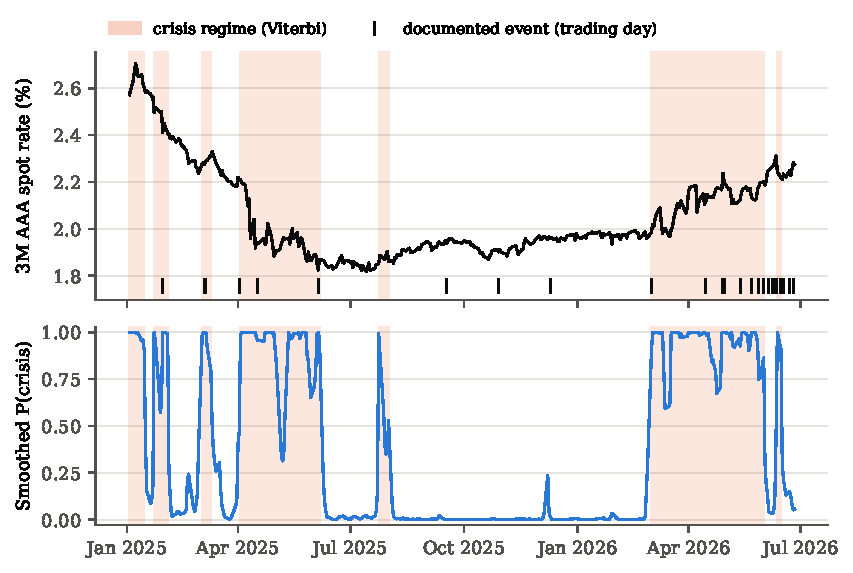
\includegraphics[width=\textwidth]{figures/fig1_regime_path.pdf}
\caption{Regime path. Top: 3-month AAA spot rate; ticks mark the trading days to which the \NEvents{} documented events are assigned (\NEventDays{} distinct days). Bottom: smoothed probability of the crisis regime. Shading: crisis regime of the Viterbi path. Source: ECB statistics; own computations.}
\label{fig:path}
\end{figure}

\begin{table}[t]
\centering\small
\caption{Model selection. Stage~1: HMM on the \NDays{} daily factor changes. Stage~2: AR(1) models of the 3-month rate on the same \NPairsKept{} within-regime pairs, conditional on the Viterbi path. BIC $=-2\ln L+k\ln n$; smaller is better. The Stage~2 comparison does not count the regime path as a parameter; its penalty is part of Stage~1. $\ln L$ and BIC are comparable only within a stage.}
\label{tab:bic}
\begin{tabular}{llrrrr}
\toprule
Stage & Model & $k$ & $n$ & $\ln L$ & BIC \\
\midrule
\tabinput{tables/tab_bic.tex}
\bottomrule
\end{tabular}
\end{table}

The one-sided check against the crisis tags supports a statement about a period, not about days. Within the tagged window of \NWindowDays{} trading days, \NTagsTD{} of which carry a tag, the smoothed crisis probability exceeds 0.5 on every one of the \NWinAprMay{} days in April and May 2026 but on only \NWinJuneHit{} of the \NWinJune{} days in June, although \NTagJune{} of the June days are tagged; over the full sample, it does so on \BaseAllPct\% of the days. The model thus marks April and May as a crisis period, tagged or not, and returns to the calm regime in June while the tags continue; it does not specifically pick out the tagged days.

\subsection{Question (a): no significant event correspondence}

\begin{table}[t]
\centering\small
\caption{Exact rotation test: all twelve registered cells. Transitions: days on which the Viterbi state changes, or on which the smoothed crisis probability crosses 0.5. Events: all documented events, or one per episode (Section~\ref{sec:rotation}). Mask: number of trading days within $\pm k$ trading days of a transition. $T_{\mathrm{obs}}$: events on masked days; $E[T\mid H_0]$: its mean over all \NDays{} circular shifts; $p$: exact, share of shifts with $T\ge T_{\mathrm{obs}}$. Only the bold (primary) cell is tested against $\alpha=0.05$; the other eleven are robustness checks whose $p$-values are reported without a test decision.}
\label{tab:rotation}
\begin{tabular}{llrrrrrr}
\toprule
Transitions & Events & $k$ & Mask & $T_{\mathrm{obs}}$ & $E[T\mid H_0]$ & $T_{\mathrm{obs}}/E$ & $p$ \\
\midrule
\tabinput{tables/tab_rotation.tex}
\bottomrule
\end{tabular}
\end{table}

In the primary specification, \Tobs{} events lie within two trading days of a Viterbi transition, against \ETprim{} expected under the null. The exact $p$-value is \Pprim{}, above $\alpha=0.05$. Condition (3) of the success criterion is not met, and the registered stopping rule applies: question (a) is answered with a diagnosed negative result (Section~\ref{sec:limits}).

The direction of the effect is stable. In all twelve cells, the observed count exceeds its null expectation, by factors between \RatioMin{} and \RatioMax{} (Table~\ref{tab:rotation}). Since the cells share the same events and transitions, this shows insensitivity to the specification, not independent confirmation. That a doubling of the chance level is not significant is due to the shape of the null distribution: in the primary cell it ranges from \NullMin{} to \NullMax{}, and \NullGE{} of the \NDays{} shifts reach $T\ge\Tobs$. Both series are clustered: the \NDaysJune{} trading days of June 2026 carry \NEventsJuneTD{} of the \NEvents{} events, and the transitions concentrate in the first four months of 2025 (\NSwitchEarly{} of \NSwitch) and in June 2026 (\NSwitchJune). Shifts that move the June event cluster onto the early-2025 transitions produce counts as high as the observed one: of the \NullGE{} shifts with $T\ge\Tobs$, \NHighEarly{} place the centre of the June events in the first four months of 2025. This is exactly the dependence that the circular shift is meant to preserve. Placing each event independently on a random trading day, which ignores this clustering, would give a narrower null distribution (standard deviation \IndepSD{} against \NullSD{} under the circular shifts), so a small $p$-value would partly reflect that assumption rather than the data.

Of the robustness cells, \NLowP{} fall below 0.05: Viterbi with one event per episode and $k=3$ ($p=\LowPa$), and the 0.5 crossing with one event per episode and $k=3$ ($p=\LowPb$). They are reported, not promoted. Without the registration fixed beforehand, a significant headline could have been selected from these cells; with twelve overlapping specifications, isolated $p$-values below 0.05 can arise by chance even under the null.

The negative result is not evidence that events and regimes are unrelated. The matches are not confined to the June cluster: of the \Tobs{} matches, \NHitsEarly{} come from the \NEventsEarly{} events before April 2026 and \NHitsLate{} from the \NEventsLate{} events from April onwards, all of the latter close to the \NSwitchJune{} June transitions. The null distribution is wide because each series is clustered on its own, not because the observed matches are concentrated. At this sample size, significance at $\alpha=0.05$ would have required at least \TcritPrim{} matches ($p=\PcritPrim$), \RatioCritPrim{} times the null expectation; the observed \Tobs{} fall short of that. The appropriate reading is that the point estimate is consistent with the hypothesised direction, roughly twice the chance level in every specification, but the exact rotation test cannot distinguish it from chance at this sample size. However, \NRetroHits{} of the \Tobs{} matches come from events that were selected retrospectively under judgement-based criteria (Section~\ref{sec:limits}), so the point estimate itself may overstate the association.

\subsection{Question (b): no joint statement; the volatility ratio excludes one, mean reversion is imprecise}

\begin{table}[t]
\centering\small
\caption{Regime-conditional Ornstein--Uhlenbeck parameters of the 3-month rate: conditional ML point estimates and bootstrap BCa 95\% intervals ($B=2000$), conditional on the Viterbi path. $a$ in 1/year, $\sigma$ in percentage points per $\sqrt{\text{year}}$, $h=1/252$. Percentiles (lower / upper): position of the interval limits in the bootstrap distribution. Bias: bootstrap mean minus point estimate; point estimates are not bias-corrected. $z_0$: bias-correction constant; $\hat a_{\mathrm{acc}}$: acceleration. MC s.e. (lower / upper): Monte Carlo standard error of the limits (grouped jackknife, $J=10$). $^\dagger$Reported but not interpretable under the registered rule, since the interval for $a$ in the crisis regime contains zero.}
\label{tab:params}
\footnotesize\setlength{\tabcolsep}{4pt}
\begin{tabular}{lrcrrrrr}
\toprule
 & Estimate & BCa 95\% & Percentiles (\%) & Bias & $z_0$ & $\hat a_{\mathrm{acc}}$ & MC s.e. \\
\midrule
\tabinput{tables/tab_params.tex}
\bottomrule
\end{tabular}
\end{table}

The conditional ML estimates are $\hat b=\bK$ in the crisis regime and $\bR$ in the calm regime, which gives $\hat a=\aK$ and $\aR$ per year and $\hat\sigma=\sK$ and $\sR$ percentage points per square-root year (\nK{} and \nR{} pairs).

\emph{Volatility.} The ratio $\sigma_{\mathrm{crisis}}/\sigma_{\mathrm{calm}}$ is \PtsRatio{} with BCa interval [\CIsRatiolo, \CIsRatiohi], which excludes 1 (Table~\ref{tab:params}). The individual intervals, [\CIsKlo, \CIsKhi] and [\CIsRlo, \CIsRhi], do not overlap. Short-rate volatility in the crisis regime is thus estimated at about \PtsRatioRound{} times that in the calm regime, a difference that the variance-based regime definition partly implies (Section~\ref{sec:limits}).

\emph{Mean reversion.} The interval for $a$ in the crisis regime, [\CIaKlo, \CIaKhi], contains zero, so fast mean reversion, a random walk and explosive dynamics ($a<0$) are all compatible with the data; for the calm regime the interval is [\CIaRlo, \CIaRhi]. In \NbOneK{} of 2000 crisis replicates (and \NbOneR{} calm replicates) the bootstrap estimate $b^*$ is at least 1. By the registered rule, the interval for the $a$-ratio, [\CIaRatiolo, \CIaRatiohi], is reported but not interpreted; read as an interval, it would contain 1 in any case. The bootstrap mean of $a^*$ in the crisis regime is \MeanaK{}, well above the estimate of \aK{}. This reflects the downward bias of the least-squares autoregressive coefficient in short samples \citep[eq.~2.7]{tangchen2009}, which the bootstrap reproduces in its own world where $\hat b$ is the true value: the mean of $b^*$ is \MeanbK{} against $\hat b=\bK$. The bootstrap bias of $\hat a$ in Table~\ref{tab:params} is considerably smaller than the analytical leading term for a single contiguous series given in Section~\ref{sec:limits}; neither is reliable this close to a unit root, so the size of the bias remains uncertain. The lower limit for crisis $a$ falls at the \PloaK\% point of the bootstrap distribution, and the upper limit for crisis $\sigma$ at the \PhisK\% point; these limits rest on very few replicates and should be read with corresponding caution (Section~\ref{sec:bootstrap}). The limit that decides the volatility finding, the lower limit of the $\sigma$-ratio, falls at the \PlosRatio\% point and is not affected.

\emph{Joint statement.} Only the $\sigma$-ratio excludes 1. By the registered intersection--union rule, the joint statement that $(a,\sigma)$ differ across regimes is therefore not made. The regime difference in volatility is reported as an individual, descriptive finding.

\emph{Model selection.} Conditional on the regime path (Section~\ref{sec:bic2}), the regime-specific AR(1) model is preferred to a single AR(1) by a BIC difference of \DBICtwo{} (Table~\ref{tab:bic}). Since the conditional Gaussian likelihood of each regime depends only on its residual variance, part of this gain reflects the same volatility difference. Because the crisis residuals are non-normal, the Gaussian likelihood is a quasi-likelihood.

\section{Limitations and discussion}\label{sec:limits}

The limitations below are part of the result. Those that were identified only after the computation they concern are dated; none of them led to a change in a registered decision.

\paragraph{What the negative result for (a) means.} The diagnosis registered in advance applies: on this sample, Gaussian, yield-only states track statistical structure, namely volatility, rather than demonstrably economic regimes. That the inferred regimes differ mainly in volatility is in line with regime-switching term-structure models that distinguish high- and low-volatility regimes \citep{dai2006}. The diagnosis is partly a statement about power: events cluster in June 2026 and transitions in early 2025 and June 2026, so the null distribution of the rotation test is wide, and a correspondence of about twice the chance level, while consistent with the hypothesised direction, cannot be distinguished from chance (Section~\ref{sec:results}). Two features of the event record favour a positive finding and therefore do not weaken the negative one, although they qualify the point estimate: the retrospectively compiled events discussed under \emph{Validation data} below, and a possible mild circularity for events whose selection may itself reflect the market reaction. The clearest case is the German fiscal package of 5 March 2025, whose event description records the rise of the 10-year Bund yield on the day; such an event may have entered the record partly because of the yield change from which the regimes are inferred.

\paragraph{The rotation test may be liberal (identified 26 August 2026, after the test run).} \citet[Sec.~1, 2.1]{mrkvicka2020} show that their toroidal shift, of which the circular shift used here is the one-dimensional case, breaks the correlation structure at the seam, so that the statistics are not exchangeable under the null and the test rejects too often; they propose a variance correction and note that the minus (border) correction avoids the problem at the cost of discarding data. The registration, which described the seam as harmless, was not revised in the light of this later reading. Their results concern spatial random fields and point patterns; whether and how strongly they apply to a one-dimensional event count against a fixed mask was not examined here. If the test is liberal in this setting as well, the bias favours significance and therefore works against the reported non-significant result, not for it.

\paragraph{Mean reversion is weakly identified; the bootstrap is at its limit.} With $n(\hat b-1)=\LUK$ (crisis) and $\LUR$ (calm), both estimates lie in the region close to a unit root. There, the standard bootstrap of an autoregressive coefficient is invalid at $b=1$ in the model without intercept \citep[Sec.~2]{basawa1991}, the conventional bootstrap is not first-order consistent in the local-to-unity model with deterministic terms \citep[Sec.~III.B]{hansen1999}, and percentile-type intervals have poor coverage close to a unit root \citep[Sec.~IV.A, Table~1]{hansen1999}. Hansen's simulations use an AR(1) with constant and trend, so they indicate the direction rather than the size of the distortion in the constant-only model used here. None of the sources consulted establishes the BCa interval in this setting. In addition, the least-squares estimate of $b$ is biased downwards by about $(1+3b)/n$ \citep[eq.~2.7]{tangchen2009}, and for the Vasicek model the leading term of the bias of the estimated mean-reversion speed is $4/T$, with $T$ the time span in years \citep[Thm.~3.2.1]{tangchen2009}. Both expansions are derived for long samples, the second for $T\to\infty$ \citep[eq.~2.1]{tangchen2009}, and for a single contiguous series. Here $T=\nK/252$ and $\nR/252$ years, split into seven episodes per regime, far from that setting; the leading term alone amounts to \TCK{} and \TCR{} per year, larger than the estimates themselves. The expansions therefore do not fix the size of the bias here; they show only that a bias of the order of the estimates cannot be excluded. The registered design was run unchanged (decision of 28 September 2026, before the bootstrap run); methods designed for this region, such as the grid bootstrap of \citet{hansen1999}, were not added afterwards. The volatility estimate is much less affected: as $b\to1$, $\sigma=\delta\sqrt{2a/(1-b^2)}\to\delta/\sqrt h$, so $\sigma$ depends almost only on the residual scale.

\paragraph{The volatility difference is partly built in (identified 30 September 2026, after the estimation).} Stage~1 separates states mainly by the covariance of daily changes in level, slope and curvature (covariance traces \TrCalm{} and \TrCrisis{}), and the daily changes of the 3-month rate are almost fully spanned by these factor changes: a regression on them over the full sample gives $R^2=\RsqShort$ (own computation of 1 October 2026, after all other computations). A higher short-rate volatility in the crisis regime is therefore to a considerable degree what the regime definition produces; what the data add is that the excess variance of the crisis state extends to the short end. The $\sigma$-finding confirms the consistency of the two stages rather than an independent economic hypothesis, and its interval, conditional on a path selected by variance, is not a test of equal volatility. It does quantify the regime difference in the parameter that enters a regime-dependent Hull--White model.

\paragraph{Stage~2 is conditional on the regime path (identified 1 October 2026, after all computations).} All Stage~2 intervals are conditional on the Viterbi path: the bootstrap resamples within fixed regimes and does not reflect uncertainty in the classification of days, which is largest near transitions, where the smoothed probabilities are least decisive (they are decisive on \Decisive\% of the days). The pairs that span a transition are excluded, but the intervals are likely to be too narrow to this extent.

\paragraph{The interpretation rule for the $a$-ratio is stricter than its justification (identified 29 September 2026, after the bootstrap run).} The registered rule declares the $a$-ratio not interpretable if the interval of $a$ in \emph{either} regime contains zero. The cited justification covers only the denominator: a ratio's confidence set becomes unbounded when the denominator is not distinguishable from zero \citep[p.~9]{franz2007}. If only the numerator's interval contains zero, as here, the confidence set remains bounded; by the geometric construction it then contains zero. The rule was not changed. The conclusion does not depend on it, because the $a$-ratio interval contains 1 in either reading.

\paragraph{Validation data.} The crisis tags cover a window of only \NWindowDays{} of the \NDays{} trading days (\NTagsTD{} of them tagged), so every crisis day before \TagStart{} is unchecked by them: a missing tag does not mean the absence of a crisis, and the check cannot yield a false-alarm rate. The application of the four event criteria to the briefings required judgement, even though the criteria were fixed in advance. The event list was audited by rule after the first model fit but before any event--transition proximity statistic was computed; as described in Section~\ref{sec:data}, the diagnostic plot of the first fit had already overlaid the event dates on the smoothed regime probabilities, so the audit decisions were not taken blind to their visual alignment (identified 30 September 2026, after all computations). The ten events before \TagStart{}, when the daily briefings begin, were not recorded contemporaneously but compiled retrospectively from official releases and news reports (recognised as a limitation on 30 September 2026, after the test run). Seven of them are rate changes, for which the selection rule leaves little room for judgement. The other three, the German fiscal package (5 March 2025), the US tariff shock (2 April 2025) and the start of the Hormuz crisis (28 February 2026), were selected under criteria K2 and K3 with hindsight; all three lie within two trading days of a Viterbi transition and account for \NRetroHits{} of the \Tobs{} matches in the primary cell. A later check of the six events documented only by a briefing against official or agency sources (1 October 2026, after all computations) confirmed that all six occurred; one had been recorded as 7 instead of 5 June 2026, which leaves $T_{\mathrm{obs}}$ unchanged and changes $p$ from \Pprim{} to \PaltSrc{}, and corrections to the event descriptions are documented in a separate file in the repository.

\paragraph{Feature construction and information sets (identified 30 September 2026, after all computations).} The principal components are estimated on standardised yield levels over the full sample. The factor changes, and with them even a filtered regime path, therefore use full-sample information through the standardisation and the loadings, and the HMM parameters are estimated on the full sample as well. For the descriptive questions of this paper this is harmless; a predictive application would have to re-estimate standardisation, loadings and HMM parameters recursively.

\paragraph{Scope.} The design is deliberately narrow: two regimes, since a third would be estimated from too few days; a one-factor model, to avoid confounding the regime effect with cross-sectional flexibility; euro-area data only, because the event validation is built around euro-area narratives; and regimes treated as given in Stage~2. The registered diagnosis names two remedies for further work. Misspecified HMMs tend to produce unstable, impersistent state estimates and unnecessary states \citep[Sec.~3.1]{nystrup2021}; the states here are persistent, but the crisis residuals are clearly non-normal. Jump models, which \citet{nystrup2021} present as an alternative to HMMs, and heavy-tailed emissions such as a Student-$t$ HMM, which has been used, in a genomics application, to prevent outliers from producing spurious state changes \citep[as reported in][p.~11]{nystrup2021}, are therefore the natural robustness checks. The natural extension of the estimation stage is a fully integrated, Markov-modulated Hull--White model in which the latent state drives the SDE parameters and both are estimated jointly.

\paragraph{Reproducibility.} The yield data were obtained from the ECB series with a download script; since published data can be revised, the repository contains the exact file used. The random seed is fixed, the Viterbi path is identical across \NStarts{} initialisations, and every estimate and test statistic in this paper is generated from the project files by a script rather than typed. As noted in Section~\ref{sec:prereg}, the chronology of registered decisions rests on dated documents and file timestamps, not on a version-control history.

\section{Conclusion}\label{sec:conclusion}

A two-state Gaussian HMM on daily changes of euro-area yield-curve factors finds two persistent regimes that are clearly separated in volatility. Question (a), whether these regimes coincide with documented events more than by chance, is not answered in the affirmative: the pre-registered test does not reject chance ($p=\Pprim$), although the observed correspondence is about twice the chance level in every specification, a figure that events selected with hindsight may inflate; the test is too weak on about 18 months of data to separate this from the clustering of events and transitions. Question (b) receives a partial answer: short-rate volatility is estimated at about \PtsRatioRound{} times that in the calm regime, a difference that the variance-based regime definition partly implies, while the mean-reversion speed cannot be estimated precisely enough to compare, so the joint claim is not made. Conditional on the regime path, BIC prefers the regime-specific model, partly through the same volatility difference. The results suggest that, on such data, regime-dependent volatility is the part of a regime-switching short-rate model that the data support, although not independently of the regime definition, and that tying statistical regimes to economic events would require a longer sample with more events and transitions. Methodologically, the study illustrates what the pre-registration protected against: two of the twelve registered cells would have offered a significant headline.

\section*{Use of AI assistance}
\addcontentsline{toc}{section}{Use of AI assistance}
The research questions and all registered design decisions are the author's. AI assistance (Anthropic's Claude, the only AI tool used, accessed through the Claude app, Claude Code and Cowork throughout the project) was used for literature search and verification, for methodological suggestions, which the author evaluated and decided on, for parts of the code and for drafting this text. The event record was compiled with AI assistance: candidate events were researched by the AI assistant, partly from daily market briefings it generated from news sources, and selected by the author together with the AI assistant under the criteria K1--K4. The Stage~1 model, the rotation test and the Stage~2 point estimates were implemented by the author, following task plans prepared by the AI assistant. The rotation test and the Stage~2 point estimates were cross-checked by independent AI-written implementations; the Stage~1 fit was reproduced by AI-written scripts using the same library. For the bootstrap and the Stage~2 BIC, both implementations whose results are compared were AI-written, on a design fixed by the author, and reviewed line by line by the author. The script that generates the tables, the figure and the numbers in the text is AI-written. This text was drafted with AI assistance from the author's project documentation; the author is responsible for its content.

\section*{Code and data availability}
\addcontentsline{toc}{section}{Code and data availability}
Code, the yield data (Source: ECB statistics), the event record and the crisis tags, all result files and the dated design documents, including the audits of the event record, are available in the public repository \url{https://github.com/Lvm2906/RS-HW}. The daily briefings from which the later events and the crisis tags were taken are AI-generated summaries of copyrighted news sources and are not redistributed; the script that extracts the tags from them is included. The modification times of the project files, recorded before the first commit, are listed in the repository. The README lists the package versions used, except for two packages whose versions were not recorded on the author's machine, and the steps to reproduce every table and figure.

\bibliographystyle{plainnat}
\bibliography{refs}

\end{document}
